To find the optimal algorithm for handwritten digit recognition the K-NN and Decision trees algorithms will be compared.
In this section the algorithms are compared based on training, classification and success rate.

\subsection{Training}
The K-NN algorithm is a direct comparison of the train data and the test data.
Thus it does not need to build a model.
Instead the K-NN algorithm relies on preprocessing the data.
In terms of speed this is faster as the test data will be preprocessed with the same methods as well.

The decision tree algorithm has to build a model of the training data. 
As shown in section \ref{sec:tree} building the decision tree from the training data of 19 people takes 2000 seconds.
\todo[inline]{find out how much time it takes to build the optimal tree}
It can be assumed that the model will only be built once as a setup and thus the impact of building the model should not be a determining factor.

\subsection{Classification}
A big difference between K-NN and decision trees are that K-NN is a brute force comparison.
In figure \ref{fig:algo_compare_timing} is the timing of classification compared.
400 digits of each class were classified using 19 peoples data as training.
Here it is clear that K-NN takes more time to classify the digits.
The tree removes half of the potential comparisons with each decision split which makes it scale well on large datasets.

\begin{figure}[H]
\centering
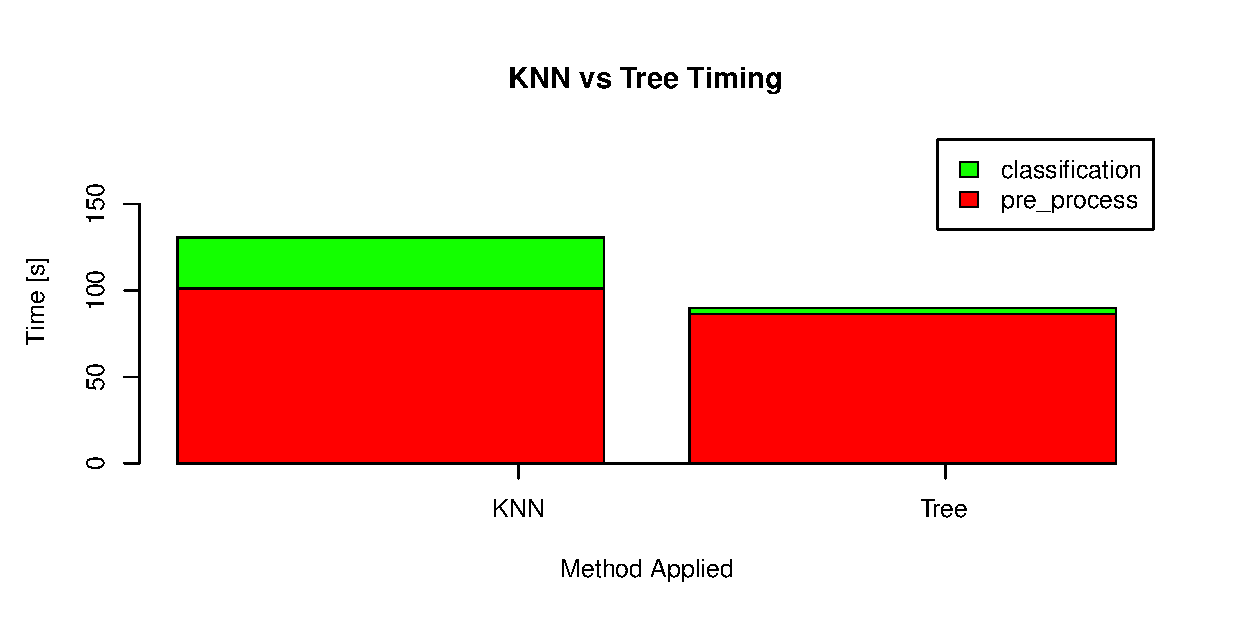
\includegraphics[width=\textwidth]{graphics/algo_compare_timing}
\label{fig:algo_compare_timing}
\end{figure}
% tree_vs_knn_timing.R

\subsection{Success Rate}
The performance of a classification method is measured in the success rate on the test data.
In figure \ref{fig:success_comparison_hard} is the algorithms success rate of the hard problem shown.
It can be seen that K-NN algorithm has a better overall performance.

\begin{figure}[H]
\centering
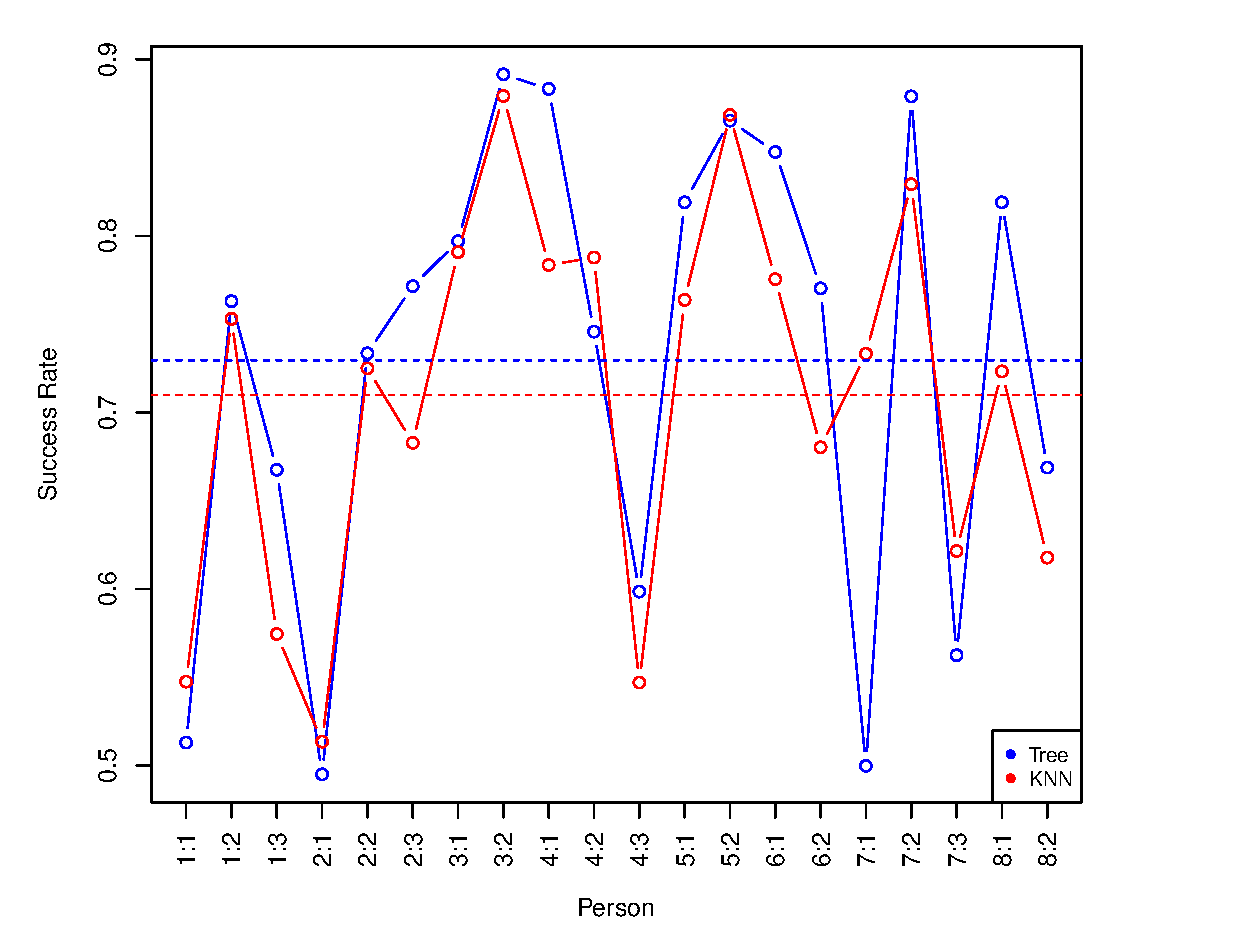
\includegraphics[width=\textwidth]{graphics/success_comp_hard}
\caption{Success for different group members.}
\label{fig:success_comparison_hard}
\end{figure}

